\section{Introduction}
Forging is a core forming process in advanced equipment manufacturing.
As illustrated in Fig. \ref{fig:forging_press}, the workpiece undergoes
plastic deformation under compression between the upper and lower dies.
The forging speed, as a pivotal parameter, influences the
thermo-mechanical response and material dynamic softening behavior by
controlling the strain rate, thereby playing a decisive role in both
forming quality and efficiency.

However, this process is highly nonlinear, dynamically fast-changing,
and its internal state is often unmeasurable, making speed
decision-making a challenging open-loop control problem.
Traditional constant-speed strategies struggle to fully exploit material
dynamic softening, while variable-speed strategies present their own
difficulties: excessively high speeds can cause stress concentration and
damage, while excessively low speeds lead to increased deformation
resistance due to billet cooling, heightening the risk of cracking.
Consequently, rational planning of a speed profile to balance efficiency
and quality is of critical importance.

\begin{figure}[htbp]
\centerline{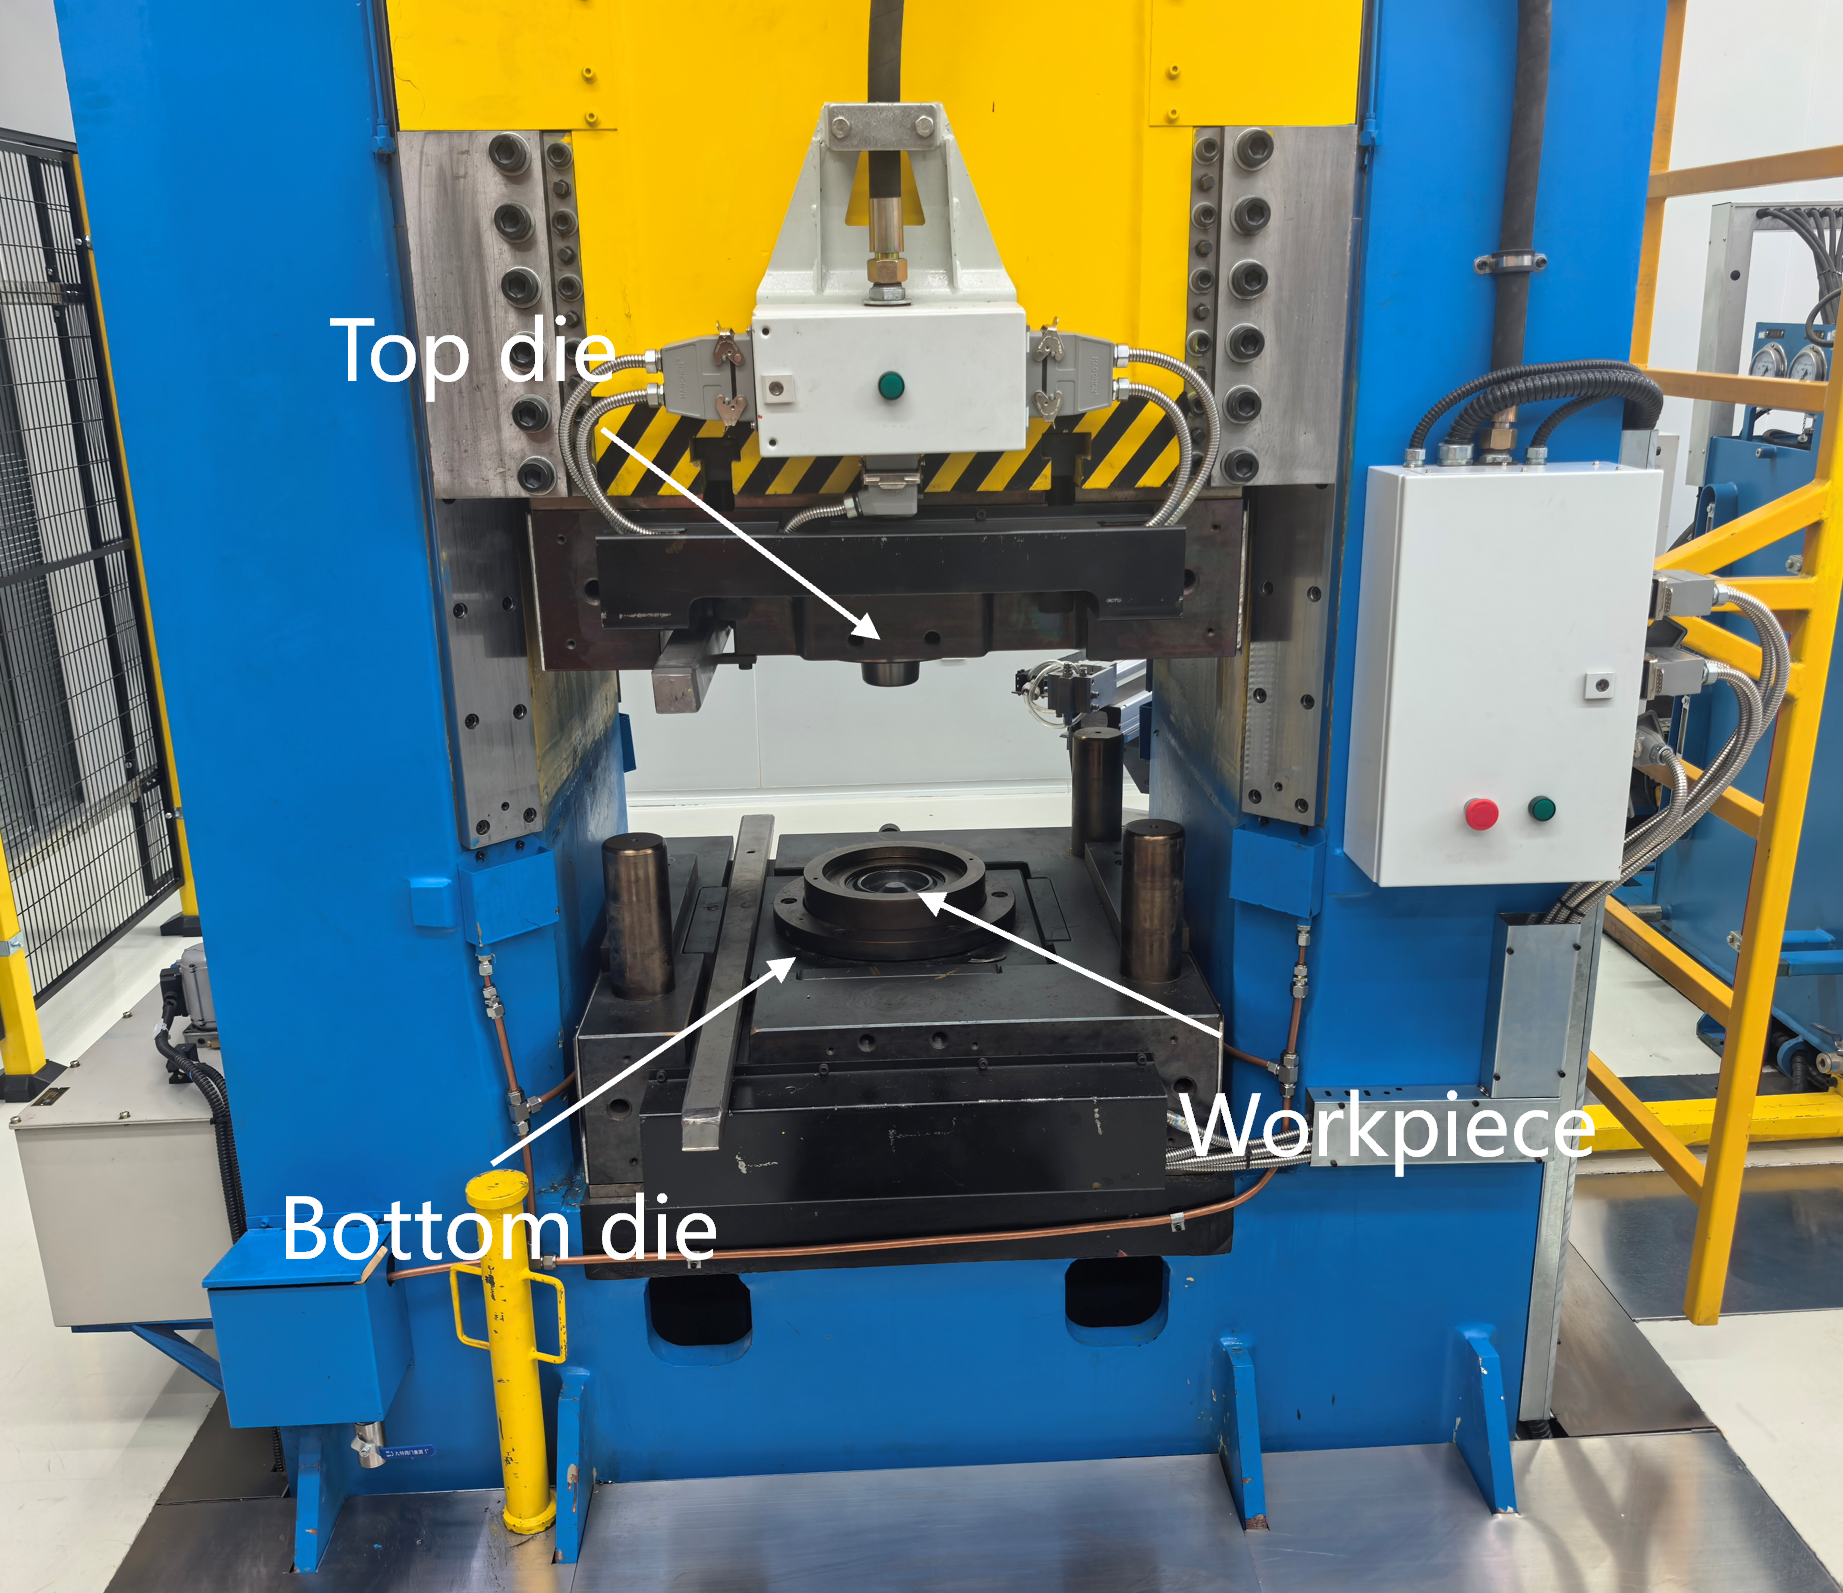
\includegraphics[width=\linewidth]{forging_press.png}}
\caption{Forging press.}
\label{fig:forging_press}
\end{figure}

% 为充分利用铝合金的动态软化特性\cite{lin2011critical}，本文提出"先慢后快"的变速策略：在变形初期以较低速度抑制应力集中，待材料进入软化阶段后逐步提高速度以兼顾效率。然而，实现该策略需解决高维非线性系统的优化控制难题。传统方法如模型预测控制(MPC)\cite{kouvaritakis2016model}优化速度慢，迭代学习控制(ILC)\cite{ahn2007iterative}依赖工况重复性，难以适应锻造过程的波动。
% 近年来，强化学习(RL)在机器人控制\cite{hafner2020mastering}等领域展现出强大潜力。例如，Stendal与Bambach\cite{stendal2024developing}提出了融合强化学习与有限元分析的协同仿真框架，用于钛铝合金塑性成形过程的智能控制，然而，该方法依赖于在线实时调整工艺参数的反馈机制，而真实锻造过程中显著的系统响应延迟使得此类闭环策略难以稳定实施；Dharmadhikari等人\cite{dharmadhikari2023reinforcement}则开发了基于无模型Q学习的强化学习框架，实现了增材制造工艺参数的自主优化。
% 这些方法均需在真实环境或仿真中进行在线学习。然而，真实锻造环境试验成本高、系统响应延迟长、设备操作风险大，完全不具备在线探索学习的条件，因此上述工作缺乏工程适用性。

% 离线强化学习(ORL)\cite{levine2020offline}通过基于历史数据学习策略，有效规避了在线交互的风险。DeepThermal\cite{zhan2022deepthermal}采用基于模型的ORL框架实现了发电机组的安全控制，Yuan等\cite{10705802}提出的时序批约束Q学习算法在浓密机控制中取得成效，验证了ORL在工业过程中的可行性。

% 然而，将离线强化学习应用于高维非线性锻造过程仍面临两大挑战：现有方法多依赖低维观测数据，难以准确表征锻造的多物理场耦合演化过程，亟需发展轻量化代理模型以替代昂贵的有限元仿真。此外，锻造设备的锻压速度属于高维连续动作，这导致策略学习与优化的复杂度显著提升。


% 针对上述挑战，本研究围绕铝合金锻造场景，重点研究：1.如何建立预测温度场、应力场与位移场全时域演化的高精度、高效率代理模型；2.如何基于离线强化学习，实现锻压速度曲线的低维参数化表征与开环优化，以生成满足多目标约束的高效设定曲线。主要贡献如下：




% 1．提出了基于深度算子网络的锻压过程代理模型架构，能够高精度、高效率地预测应力场、位移场等多物理场的时空演化过程，为策略学习提供了高效数据生成器。

% 2．提出了面向锻造场景多约束、多优化目标特点的离线安全强化学习范式。构建能够直接生成最优锻造速率曲线的优化控制器。
To fully exploit the dynamic softening characteristics of aluminum alloys
\cite{lin2011critical}, this paper proposes a "slow-then-fast"
variable-speed strategy. This approach employs a lower speed at the
initial deformation stage to mitigate stress concentration, and
subsequently increases the speed as the material enters the softening
stage to enhance efficiency. However, implementing this strategy
requires solving the optimal control problem of a high-dimensional
nonlinear system. Conventional methods, such as model predictive
control (MPC) \cite{kouvaritakis2016model}, suffer from slow
optimization speeds, while iterative learning control (ILC)
\cite{ahn2007iterative} relies on operating condition repeatability,
making them unsuitable for handling fluctuations in the forging process.

Recently, reinforcement learning (RL) has demonstrated considerable
potential in domains like robotic control \cite{hafner2020mastering}.
For instance, Stendal and Bambach \cite{stendal2024developing} developed
a co-simulation framework integrating RL with finite element analysis
for the intelligent control of Ti-Al alloy plastic forming. However,
their method depends on a feedback mechanism for online parameter
adjustment, which is challenging to implement stably in real forging due
to significant system response delays. Dharmadhikari et al.
\cite{dharmadhikari2023reinforcement} devised a model-free Q-learning
framework for autonomous optimization of additive manufacturing
parameters.

These methods, however, require online learning in either real or
simulated environments. Conducting online exploration in real forging is
impractical due to high costs, long delays, and operational risks, thus
limiting the engineering applicability of the aforementioned approaches.

Offline reinforcement learning (ORL) \cite{levine2020offline} overcomes
this limitation by learning policies directly from historical datasets,
effectively avoiding the risks of online interaction. For example,
DeepThermal \cite{zhan2022deepthermal} employed a model-based ORL
framework for safe control of power units, and Yuan et al.
\cite{10705802} achieved effective control in thickener operation with a
temporal batch-constrained Q-learning algorithm, validating ORL's
feasibility in industrial processes.

Nevertheless, applying ORL to high-dimensional nonlinear forging poses
two major challenges. First, existing methods often rely on
low-dimensional observational data, which is insufficient to characterize
the coupled multi-physics evolution, necessitating a lightweight
surrogate model to replace costly finite element simulations. Second,
the forging speed constitutes a high-dimensional continuous action,
significantly increasing the complexity of policy learning and
optimization.

To address these challenges, this study focuses on aluminum alloy
forging and investigates: 1) establishing a high-precision and efficient
surrogate model for predicting the full-time evolution of temperature,
stress, and displacement fields; and 2) leveraging ORL to achieve
low-dimensional parameterization and open-loop optimization of the speed
profile, generating an efficient set-point curve that satisfies multiple
constraints. The main contributions are as follows:

1. We propose a surrogate model architecture for the forging process
based on the deep operator network, which enables highly accurate and
efficient prediction of the spatiotemporal evolution of multi-physics
fields (e.g., stress and displacement), serving as an efficient data
generator for policy learning.

2. We propose an offline safe RL paradigm tailored for the
multi-constraint, multi-objective nature of forging. An optimal control
agent is developed to directly generate the optimal forging speed curve.

The overall framework of this research is illustrated in
Fig. \ref{fig:framework}. It consists of two stages: a point-cloud world
model is first learned from simulation data to act as a fast and
differentiable environment, and a model-based policy is then trained
within this environment to generate the forging speed curve.

\begin{figure}[htbp]
\centerline{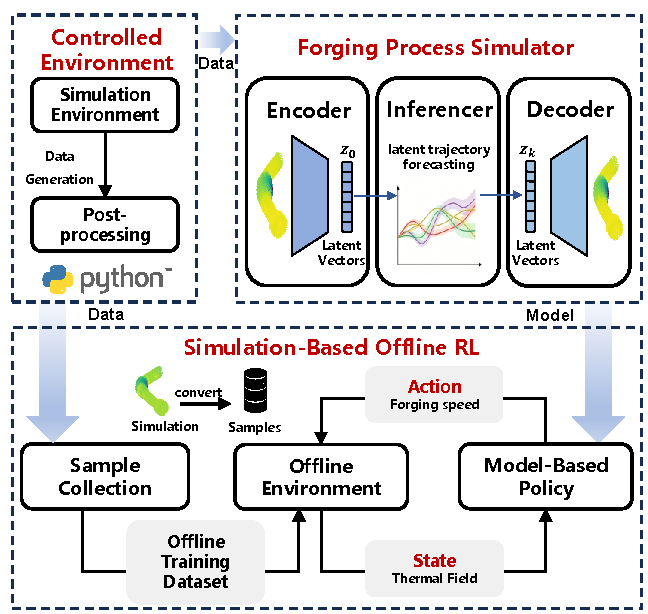
\includegraphics[width=\linewidth]{frame-1.pdf}}
\caption{The framework of this research.}
\label{fig:framework}
\end{figure}
